\documentclass[a4paper,10pt]{article} % Default font size and paper size

%{{{ Packages & Includes
%\usepackage{xunicode,xltxtra,url,parskip} % Formatting packages
\usepackage{url,parskip} % Formatting packages
\usepackage{graphicx}
\usepackage{adjustbox}
\usepackage{multirow}

\usepackage[usenames,dvipsnames]{xcolor} % Required for specifying custom colors

%\usepackage[big]{layaureo} % Margin formatting of the A4 page, an alternative to layaureo can be \usepackage{fullpage}
% To reduce the height of the top margin uncomment: \addtolength{\voffset}{-1.3cm}
%\usepackage[left=2cm,right=2cm,top=1.5cm,bottom=1.5cm]{geometry}
\usepackage[left=1.5cm,right=1.5cm,top=1.5cm,bottom=1.5cm]{geometry}
\usepackage[pdfa]{hyperref} % Required for adding links	and customizing them
\definecolor{linkcolour}{rgb}{0,0.2,0.6} % Link color
\hypersetup{colorlinks,breaklinks,urlcolor=linkcolour,linkcolor=linkcolour} % Set link colors throughout the document
\usepackage{array}
\usepackage{ragged2e}
\newcolumntype{R}[1]{>{\raggedleft\let\newline\\\arraybackslash\hspace{0pt}}m{#1}}
\newcolumntype{L}[1]{>{\raggedright\let\newline\\\arraybackslash\hspace{0pt}}m{#1}}
\newcolumntype{C}[1]{>{\centering\let\newline\\\arraybackslash\hspace{0pt}}m{#1}}

\usepackage{titlesec} % Used to customize the \section command
\titleformat{\section}{\scshape\raggedright}{}{0em}{}[\titlerule] % Text formatting of sections
\titlespacing{\section}{3pt}{3pt}{3pt} % Spacing around sections
%}}}

% Variable Definition
\newcommand\columnWidth{12.5cm}

\begin{document}

\pagestyle{empty} % Removes page numbering

\section{Personal Information}

\begin{table}[ht]
\begin{minipage}{0.77\linewidth}
    \begin{tabular}{L{1.75cm}p{3cm}p{2cm}L{1.4cm}L{1.5cm}p{1.05cm}C{1.5cm}}
        Full Name: & \textbf{Carlos Segarra} & & \multicolumn{2}{l}{\textbf{Languages:}} & & \multirow{2}{*}{\href{https://github.com/csegarragonz}{\XeTeXLinkBox{
\includegraphics[height=0.5cm]{img/git.png}}}}\\
        Birthday: & 09/06/1996 & & Spanish: & Native & & \\
        Residence: & Barcelona, Spain & & Catalan: & Native & & \multirow{2}{*}{\href{https://www.linkedin.com/in/carlossegarrag/}{\XeTeXLinkBox{
\includegraphics[height=0.5cm]{img/linkedin.jpg}}}}\\
        Website: & \href{https://carlossegarra.com}{carlossegarra.com} & & English: & C2 & &\\
        Mail: & \small{\href{mailto:carlossegarragonzalez@gmail.com}{carlossegarragonzalez@gmail.com}} & & French: & Fluent & & \multirow{2}{*}{\href{https://scholar.google.com/citations?user=U0KR_0cAAAAJ&hl=en}{\XeTeXLinkBox{
\includegraphics[height=0.5cm]{img/scholar.png}}}}\\
        Phone: & +34 699 20 89 00 & & German: & A2 & &
    \end{tabular}
\end{minipage}\hfill
\begin{minipage}{0.2\linewidth}
\centering
%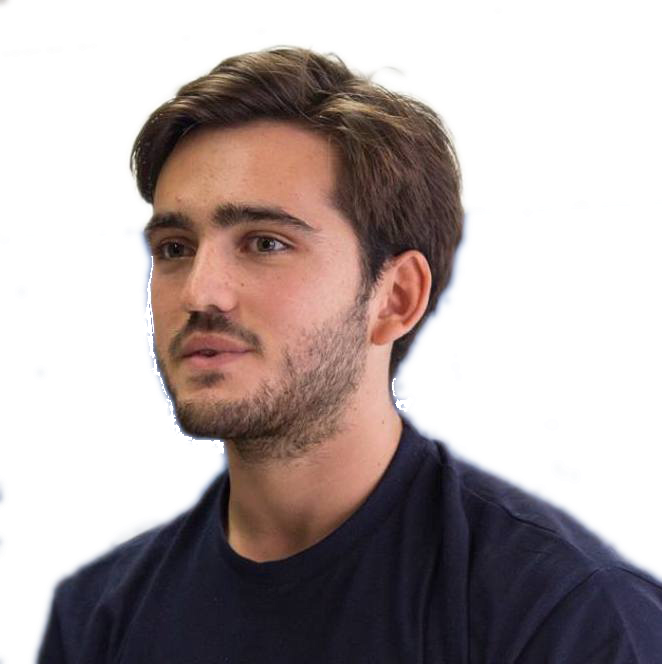
\includegraphics[width=2.5cm]{carlos_portrait.png}
{%
\setlength{\fboxsep}{0pt}%
\setlength{\fboxrule}{0.7pt}%
\fbox{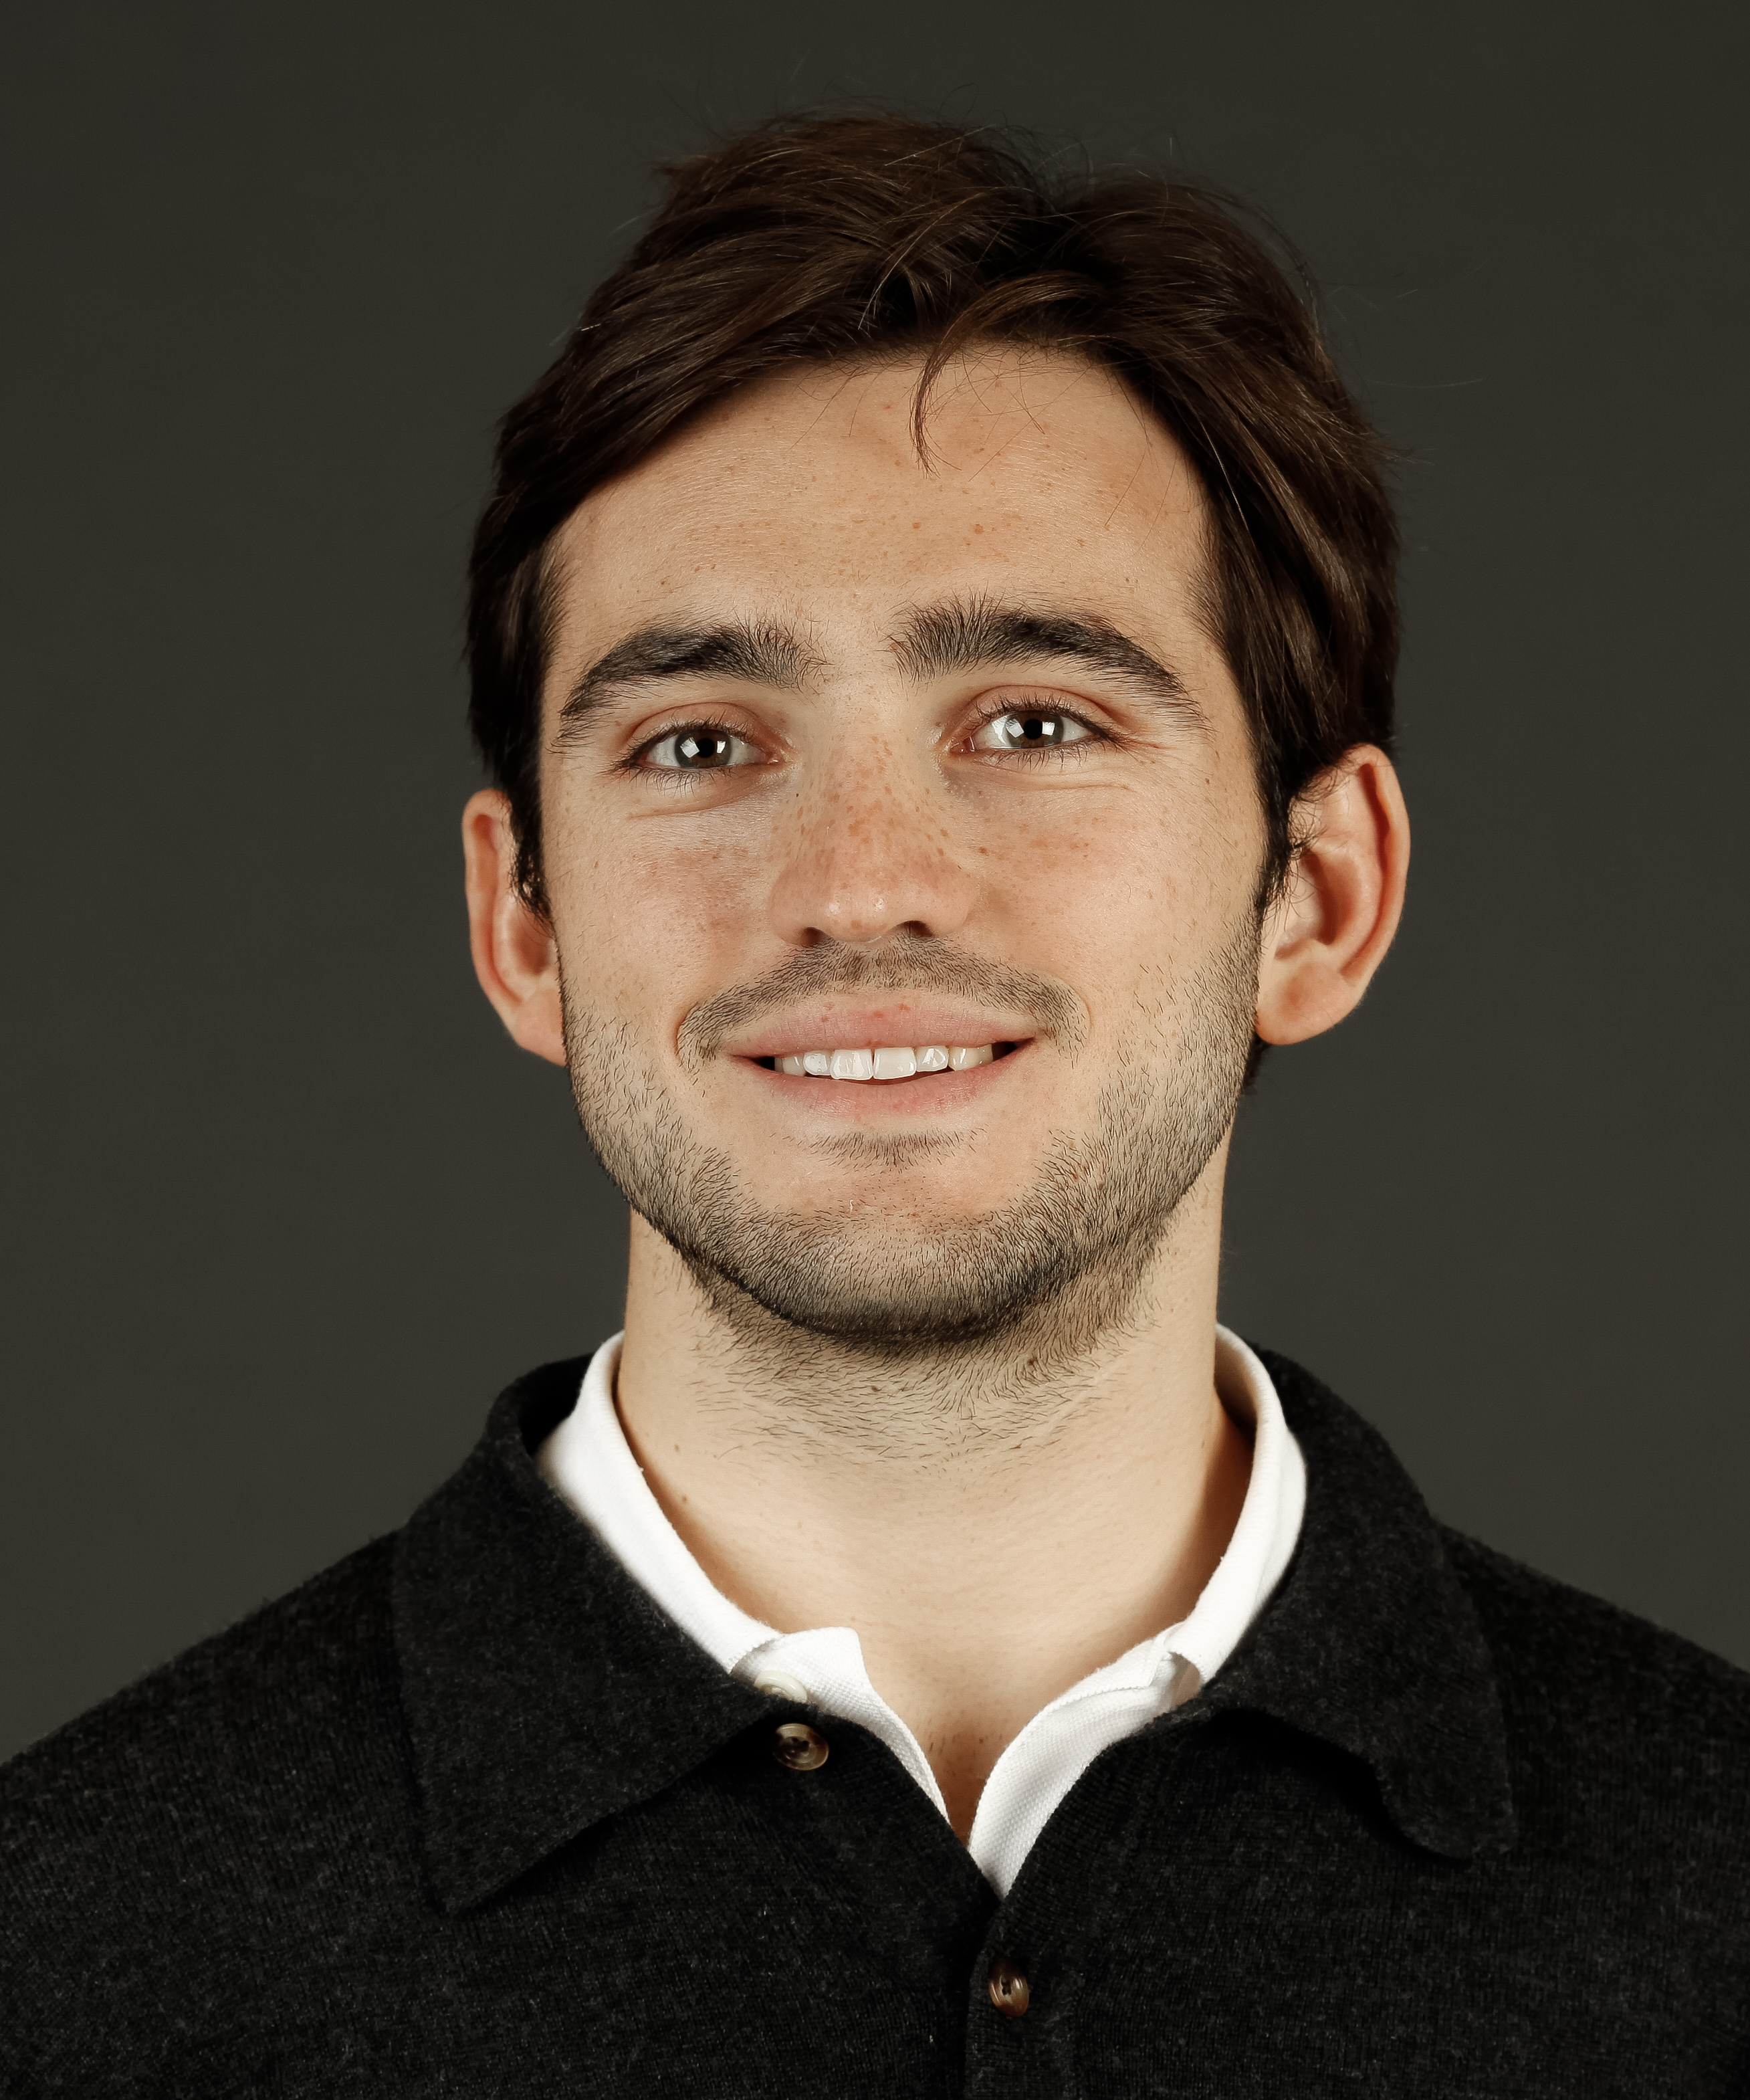
\includegraphics[width=2.1cm]{csem_img.jpg}}%
}%
\end{minipage} 
\end{table}

\section{Short Bio}
\begin{tabular}{p{\dimexpr1.5cm+15.5cm}}
    I am a MSc student in advanced mathematics at the School of Mathematics from the Technical University of Catalonia, in Barcelona, Spain.
    I am focusing on graph theory, combinatorics and cryptography.
    Further, I also attend courses on distributed systems, concurrency, and networking from the Master in Research in Informatics.
    In fall 2020, I will start a PhD in Computer Science at the Imperial College in London under the supervision of Prof. Peter Pietzuch.
    At the moment, I collaborate with the Computer Architecture Department in my home university and with the Complex Systems Group of the Universit\'e de Neuch\^atel (Switzerland).
    My main research interests are systems and security, with a strong mathematical foundation.
\end{tabular}

\section{Publications}
\begin{tabular}{p{\dimexpr1.5cm+15.5cm}}
    \textit{(Submitted)} C. Segarra, R. Delgado-Gonzalo, and V. Schiavoni, \textbf{\textit{"Hardening IoT Brokers with MQTT and TrustZone for Secure Edge-based Pub/Sub Middleware"}}. Systems Conference Ranked A. \\[3pt]
    P. Gouveia, J. Neves, C. Segarra, L. Liechti, S. Issa, V. Schiavoni, and M. Matos, \textbf{\textit{"KOLLAPS: Decentralized and Dynamic Topology Emulation"}}. EuroSys'20. \\[3pt]
    C. Segarra, R. Delgado-Gonzalo, and V. Schiavoni, \textbf{\textit{"MQT-TZ: Secure MQTT Broker for Biomedical Signal Processing on the Edge"}}. MIE 2020, Geneva, Switzerland. May 19-20, 2020. \\[3pt]
    C. Segarra, E. Muntan\'e, M. Lemay, V. Schiavoni, and  R. Delgado-Gonzalo, \textbf{\textit{"Secure Stream Processing for Medical Data"}}. IEEE EMBC'19, Berlin, Germany, July 23-27, 2019. \\[3pt]
    C. Segarra, R. Delgado-Gonzalo, M. Lemay, P-L. Aublin, P. Pietzuch, and V. Schiavoni, \textbf{\textit{"Using Trusted Execution Environments for Secure Stream Processing of Medical Data"}}. DAIS'19, Copenhagen, Denmark, June 17-21, 2019. \\
\end{tabular}

\section{Education}

\begin{tabular}{R{1.5cm}|p{\columnWidth}L{2cm}}	
    \textsc{\textit{Cond.}} & PhD in \textbf{\textsc{Computer Science}} (Sup. Prof. Peter Pietzuch) & \multirow{2}{*}{\href{https://mamme.masters.upc.edu/en}{\XeTeXLinkBox{
\includegraphics[width=1.5cm]{img/logo_imperial.png}}}} \\ 
    \textsc{10/2020} & \small{\emph{Large-Scale Data \& Systems Group - Imperial College London}, IMP} & \\
     & \footnotesize{
         PhD in Computer Science at the Large-Scale Data \& Systems Group of the Imperial College in London under the supervision of Professor Peter Pietzuch.
         I will work on secure, high-performance, and scalable containers for large-scale systems.
         Acceptance is conditional until I graduate from my MSc in July 2020.
     } &
\end{tabular}

\begin{tabular}{R{1.5cm}|p{\columnWidth}L{2cm}}	
    \textsc{\textit{Current}} & Master in \textbf{\textsc{Advanced Mathematics and Mathematical Engineering}}  & \multirow{2}{*}{\href{https://mamme.masters.upc.edu/en}{\XeTeXLinkBox{
\includegraphics[width=1.5cm]{img/upc-long-noletter.png}}}} \\ 
    \textsc{09/2019} & \small{\emph{School of Mathematics and Statistics - Technical University of Catalonia}, UPC} & \\
     & \footnotesize{
         MSc in Advanced Mathematics with a focus in Discrete Mathematics and Algorithms.
         Relevant courses cover: Graph Theory, Codes and Cryptography, and Combinatorics.
         I am also enrolled to courses from the Master in Research in Informatics (MIRI-UPC).
         Relevant courses cover: Concurrency, Parallelism, and Distributed Systems, Multiprocessors Architecture, and Decentralized Systems.
         Graduation is expected for July 2020.
     } &
\end{tabular}

\begin{tabular}{R{1.5cm}|p{\columnWidth}L{2cm}}	
    \textsc{05/2019} & Bachelor's degree in \textbf{\textsc{Mathematics}} & \multirow{2}{*}{\href{https://fme.upc.edu/en}{\XeTeXLinkBox{
\includegraphics[width=1.5cm]{img/upc-long-noletter.png}}}} \\  
    \textsc{09/2014} & \small{\emph{School of Mathematics and Statistics - Technical University of Catalonia}, UPC} & \\
     & \footnotesize{
         BSc in Mathematics within a double degree program in the Interdisciplinary Higher Education Center (CFIS) at the UPC.
         Relevant coursework covers real and complex analysis, statistics, probability and graph theory, combinatorics and algorithms.
     } &
\end{tabular}

\begin{tabular}{R{1.5cm}|p{\columnWidth}L{2cm}}	
    \textsc{05/2019} &  Bachelor`s degree in \textbf{\textsc{Telecommunications Science and Technology}} & \multirow{2}{*}{\href{https://www.ac.upc.edu/en}{\XeTeXLinkBox{
\includegraphics[width=1.5cm]{img/upc-long-noletter.png}}}} \\  
    \textsc{09/2014} & \small{\emph{Technical University of Catalonia}, UPC} & \\
     & \footnotesize{
         BSc in Telecommunications Engineering within a double degree program in the Interdisciplinary Higher Education Center (CFIS) at the UPC.
         Relevant coursework covers networking and concurrency, digital and analogical communications and real time digital signal processing.
     } &
\end{tabular}
\section{Work Experience}
%
\begin{tabular}{R{1.5cm}|p{\columnWidth}L{2cm}}
    \emph{Current} & Research Collaborator at the \textbf{\textsc{Technical University of Catalonia}} & \multirow{2}{*}{\href{https://www.ac.upc.edu/en}{\XeTeXLinkBox{
\includegraphics[width=1.5cm]{img/upc-long-noletter.png}}}}\\
    \textsc{10/2019} & \small{\emph{Computer Architecture Department, School of Informatics} - Sup. Jordi Guitart, PhD} & \\ 
    & \footnotesize{
        Research collaborator with the Computer Architecture Department (DAC) of the School of Informatics (FIB) of the Technical University of Catalonia (UPC) in Barcelona, Spain. 
        Under the supervision of Jordi Guitart, we work on live migration of containers with the goal of performing live migrations of container clusters.
        To perform migrations we rely on Checkpoint Restore In Userspace (CRIU) technology.}
\end{tabular}

\begin{tabular}{R{1.5cm}|p{\columnWidth}L{2cm}}
    \emph{12/2019} & Research Assistant at the \textbf{\textsc{Universit\'e de Neuch\^atel}} & \multirow{2}{*}{\href{https://www.unine.ch/iiun/home/chaires-de-recherche/systemes-complexes.html}{\XeTeXLinkBox{
\includegraphics[width=2cm]{img/unine}}}}\\
    \textsc{08/2019} & \small{\emph{Complex Systems Group, Institut d'Informatique} - Sup. Valerio Schiavoni, PhD} & \\ 
    & \footnotesize{
        Research collaborator with the Complex Systems Group from the UniNe.
    Under the supervision of V. Schiavoni, we worked on \textsc{Kollaps}, an emulation platform for distributed applications.
    We emulated arbitrary topologies basing on their end-to-end properties: bandwidth, jitter, latency, and packet loss. 
    Dynamic link behaviours are also emulated.
    To do so, we used traffic control functionalities available in the Linux Kernel. 
    For the emulated applications we relied on Docker containers and orchestrators such as Swarm and Kubernetes.
    In parallel, we worked on benchmarking of Trusted Execution Environments and applications leveraging them.
    } &
\end{tabular}

\begin{tabular}{R{1.5cm}|p{\columnWidth}L{2cm}}
    \textsc{07/2019} & Trainee at the \textbf{\textsc{Swiss Center for Electronics and Microtechnology} (CSEM)} & \multirow{2}{*}{\href{https://www.csem.ch/}{\XeTeXLinkBox{
\includegraphics[width=2cm]{img/csem}}}}\\
    \textsc{10/2018} & \small{\emph{Embedded Software Group} - Sup. Ricard Delgado-Gonzalo, PhD} & \\ 
    & \footnotesize{
        Intern at the Embedded Software Division of the CSEM in Neuch\^atel, CH, where I used Trusted Execution Environments to perform privacy-preserving computations on IoT medical devices.
        Developed a distributed streaming platform on Intel SGX and a secure implementation of the MQTT broker relying on TLS and ARM TrustZone.
        I also collaborated in two H2020 EU Projects: ACTIVAGE and TABEDE.
        In the former, I was responsible of implementing part of the Security \& Privacy module and in the latter of implementing the User Control Interface, visualizing data coming from a variety of IoT devices.} &
\end{tabular}

\begin{tabular}{R{1.5cm}|p{\columnWidth}L{2cm}}
    \textsc{09/2018} & Trainee at \textbf{\textsc{Nokia Bell Labs}} & \multirow{2}{*}{\href{https://www.csem.ch/}{\XeTeXLinkBox{
\includegraphics[width=2cm]{img/bell-labs.png}}}}\\
    \textsc{06/2018} & \small{\emph{Security Group} - Sup. Matteo Signorini, PhD and Matteo Pontecorvi, PhD} & \\ 
    & \footnotesize{
        Summer intern at the the Cybersecurity department at Nokia Bell Labs in Paris-Saclay, France.
        I designed, and implemented a graph-based model to detect, cluster and classify chains of malicious transactions in the Bitcoin's Blockchain.
        By defining an abstraction layer atop the chain and an isomorphism class, we managed to identify a variety of malicious services.} &
\end{tabular}

\begin{tabular}{R{1.5cm}|p{\columnWidth}L{2cm}}
    \textsc{06/2018} & Research Student at the \textbf{\textsc{Barcelona Supercomputing Center} (BSC)} & \multirow{2}{*}{\href{https://www.csem.ch/}{\XeTeXLinkBox{
\includegraphics[width=2cm]{img/bsc.jpeg}}}}\\
    \textsc{04/2017} & \small{\emph{Workflows and Distributed Computing Group} - Sup. Rosa M. Badia, PhD} & \\ 
    & \footnotesize{
        Research student at the Workflows and Distributed Computing Group at the BSC in Barcelona, Spain.
        I developed, deployed and benchmarked a distributed implementation of the DBSCAN clustering algorithm using COMP Superscalar, a programming model for distributed computing.
        Evaluation was done in the \textit{Mare Nostrum} supercomputer.
    } &
\end{tabular}


\section{Relevant Projects}

\begin{tabular}{R{1.5cm}|p{\columnWidth}L{2cm}}	
    \textsc{\textit{Current}} &  \textbf{\textsc{Live Migration of (Distributed) Container Deployments}}  & \multirow{2}{*}{\href{https://mamme.masters.upc.edu/en}{\XeTeXLinkBox{
\includegraphics[width=1.5cm]{img/upc-long-noletter.png}}}} \\ 
    \textsc{10/2019} & \small{\emph{Computer Architecture Department (DAC)}, UPC} & \\
     & \footnotesize{
         As a research collaborator with the DAC group, I am implementing live migration for running container deployments, both standalone and in a cluster. 
         We are using checkpoint-restore techniques, relying on Checkpoint/Restore in Userspace (CRIU).
         The project involves dealing with the large CRIU codebase written in \textsc{C} and implementing the right wrappers and handlers (\textsc{C} and \textsc{Go}) to make the live migration transparent to the end user.
         Even though this is an on-going project, it is \href{https://github.com/live-containers}{available} on Github.
     } &
\end{tabular}

\begin{tabular}{R{1.5cm}|p{\columnWidth}L{2cm}}	
    \textsc{11/2019} &  \textbf{\textsc{Kollaps: Decentralized and Dynamic Topology Emulator}}  & \multirow{2}{*}{\href{http://angainor.science/}{\XeTeXLinkBox{
\includegraphics[width=1.5cm]{img/angainor.png}}}} \\ 
    \textsc{07/2019} & \small{\emph{Complex Systems Group}, IIUN} & \\
     & \footnotesize{
         As a research collaborator with the Complex Systems Group at the University of Neuch\^atel, I worked in a decentralized emulator for distributed applications.
         In collaboration with the Distributed Systems Group at the INESC-ID in Lisbon, Portugal, I was responsible for the benchmarking of the project.
         In particular, I worked with applications generating different sorts of workloads (\textit{e.g} \textsc{iPerf3} and \textsc{wrk2}) along different network topologies using different TCP congestion algorithms.
         I also replicated the results in bare metal, and in other emulation and simulation engines.
         Moving forward, we will work on implementing different bandwidth sharing models to improve the emulation accuracy.
         The architecture and the benchmarking have been accepted to EuroSys 2020, once the camera ready version is made public, code will be open-sourced.
     } &
\end{tabular}

%\begin{tabular}{R{1.5cm}|p{\columnWidth}L{2cm}}	
%    \textsc{08/2019} &  \textbf{\textsc{MQT-TZ: Hardening MQTT Brokers Using Arm TrustZone}}  & \multirow{2}{*}{\href{https://github.com/mqttz}{\XeTeXLinkBox{
\includegraphics[width=1.5cm]{img/mqttz.png}}}} \\ 
%    \textsc{01/2019} & \small{\emph{Complex Systems Group}, IIUN, University of Neuch\^atel} & \\
%     & \footnotesize{
%         During my internship at the CSEM, I implemented a hardened \texttt{mosquitto} \textsc{MQTT} broker relying on Arm TrustZone.
%         In a medical IoT environment, where multiple low-powered clients stream private user data to a gateway that bridges to the cloud, this gateway becomes a single-point of failure. 
%         To minimize the attack surface I designed, implemented, and evaluated, a MQTT broker to run on this gateway.
%         Starting from \texttt{mosquitto}'s \textsc{C} source code, I encrypted data on the application layer using \texttt{openssl} with a client specific symmetric key. 
%         Re-encryption of application data was done in the Trusted Execution Environment in the broker (TrustZone). 
%         To implement this re-encryption, I built a Trusted Application using \textsc{Op-TEE} and a secure kv-store to persist client's keys in persistent secure storage.
%     } &
%\end{tabular}

%\begin{tabular}{R{1.5cm}|p{\columnWidth}L{2cm}}	
%    \textsc{06/2018} &  \textbf{\textsc{DBSCAN for PyCOMPSs}} & \multirow{2}{*}{\href{https://github.com/bsc-wdc/compss}{\XeTeXLinkBox{
\includegraphics[width=1.5cm]{img/compss.png}}}} \\  
%    \textsc{04/2017} & \small{\emph{Workflows and Distributed Computing Group}, BSC} & \\
%     & \footnotesize{
%         As a research student at the BSC, I implemented a distributed version of the DBSCAN clustering algorithm using the Python binding of the COMPS Superscalar framework.
%         The algorithm was written in Python 2.7, amounted to several hundreds of LoC, and followed a Map/Reduce structure where the initial dataset was distributed in a pre-processing stage following a spatial proximity criterion.
%         I also benchmarked the application in the \textit{Mare Nostrum} supercomputer scaling up to thousands of cores, and implemented the deployment scripts for the different queueing protocols.
%         The \href{https://github.com/csegarragonz/DBSCAN-pyCOMPSs}{source code} is available on my Github page.} &
%\end{tabular}

\end{document}
